\documentclass[border=10pt]{standalone}

\usepackage{tikz}
\usepackage{tikzsymbols}
\usetikzlibrary{calc,patterns,shapes.geometric}

\def\centerarc[#1](#2)(#3:#4:#5){\draw[#1] ($(#2)+({#5*cos(#3)},{#5*sin(#3)})$) arc (#3:#4:#5);}

\begin{document}
	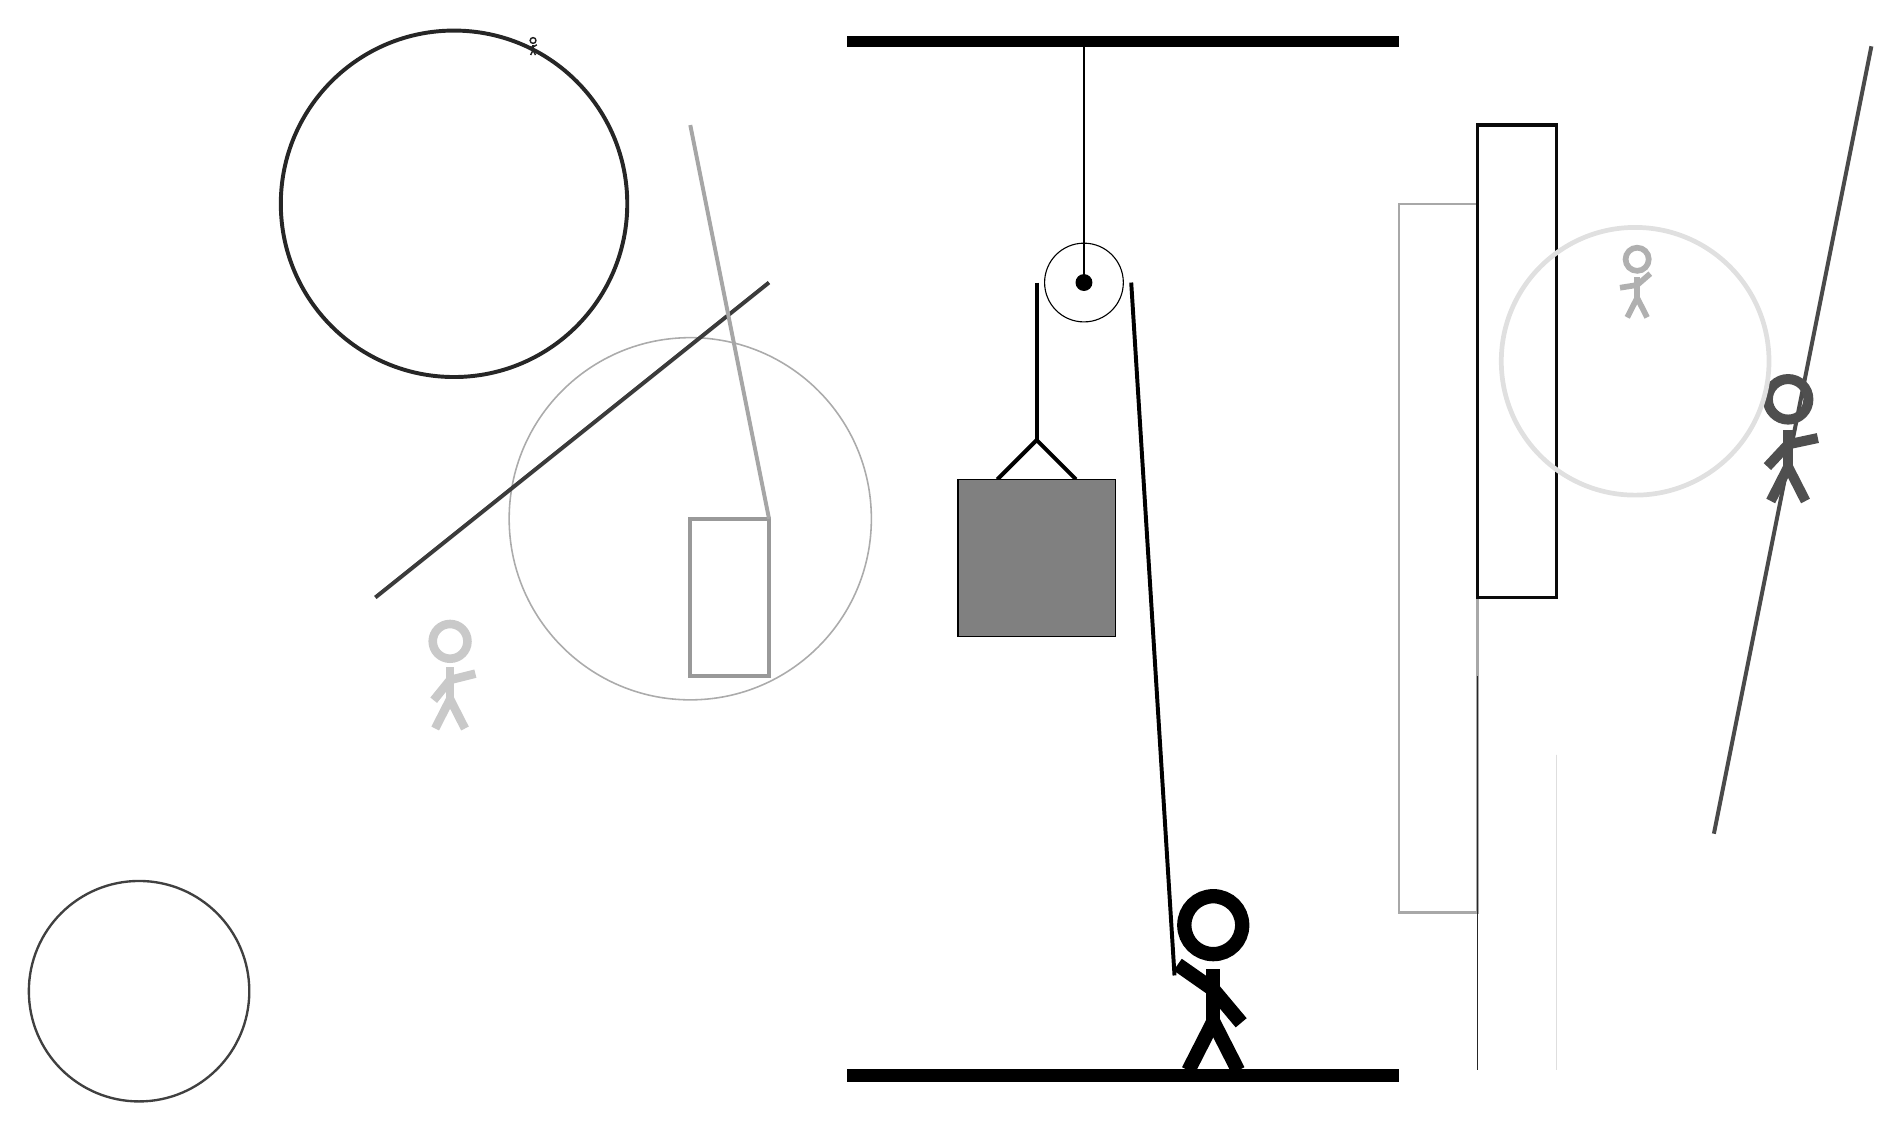
\begin{tikzpicture}
		%%%%% START %%%%%
		
		\draw[fill=black] (-2, 10) rectangle (5, 10.125);
		
		\draw (1, 7) circle (0.5);
		\draw[fill=black] (1, 7) circle (0.1);
		\draw (1, 10) -- (1, 7);
		
		\draw[line width=0.5mm] (-0.1, 4.5) -- (0.4, 5.0) -- (0.9, 4.5);
		\draw[fill=black!50] (-0.6, 4.5) rectangle (1.4, 2.5);
		
		\draw[line width=0.5mm] (0.4, 7) -- (0.4, 5.0);
		\centerarc[line width=0.5mm](1, 7)(0:180:0.6);
		\draw[line width=0.5mm](1.6, 7) -- (2.15, -1.8);
		
		\node[line width=0.2mm, color=black!31] at (8, 7) {\Strichmaxerl[4][9][41]};
		
		\draw [line width=0.3mm, color=black!75](-11, -2) circle (1.4);
		\draw[line width=0.5mm, color=black!40] (-4, 4) rectangle (-3, 2);
		\draw[line width=0.5mm, color=black!71](9, 0) -- (11, 10);
		
		\draw[line width=0.2mm, color=black!13] (7, -3) rectangle (7, 1);
		\draw[line width=0.3mm, color=black!34] (5, 8) rectangle (6, -1);
		\node[line width=0.4mm, color=black!21] at (-7, 2) {\Strichmaxerl[6][51][14]};
		\draw[line width=0.2mm, color=black!85] (6, 2) rectangle (6, -3);
		\node[line width=0.4mm, color=black!87] at (-6, 10) {\Strichmaxerl[1][3][29]};
		\node[line width=0.3mm, color=black!69] at (10, 5) {\Strichmaxerl[7][47][12]};
		\draw[line width=0.4mm, color=black!96] (6, 9) rectangle (7, 3);
		\draw [line width=0.6mm, color=black!12](8, 6) circle (1.7);
		\draw [line width=0.5mm, color=black!85](-7, 8) circle (2.2);
		\draw [line width=0.2mm, color=black!33](-4, 4) circle (2.3);
		\draw[line width=0.5mm, color=black!77](-3, 7) -- (-8, 3);
		\draw[line width=0.5mm, color=black!35](-3, 4) -- (-4, 9);
		
		
		\node at (2.6, -1.9) {\Strichmaxerl[10][-35][-50]};
		
		\draw[fill=black] (-2, -3) rectangle (5, -3.15);
		
		%%%%% END %%%%%
	\end{tikzpicture}
\end{document}